% !TEX program = xelatex
\documentclass[a4paper,10pt]{article}
\usepackage[UTF8,fontset=none]{ctex}
\usepackage{xeCJK}
\setCJKmainfont{Songti SC}
\setCJKsansfont{STHeiti}
\setCJKmonofont{Songti SC}
\usepackage[margin=2.2cm]{geometry}
\usepackage{tikz}
\usetikzlibrary{shapes.geometric, arrows.meta, positioning, calc, fit}
\usepackage{amsmath, amssymb}
\usepackage{longtable}
\usepackage{array}
\usepackage{booktabs}
\usepackage{multirow}
\usepackage{enumitem}
\usepackage{fancyhdr}
\usepackage{titlesec}
\usepackage{hyperref}
\usepackage{xcolor}
\usepackage{tabularx}

\hypersetup{
  colorlinks=true,
  linkcolor=blue!60!black,
  urlcolor=blue!60!black,
  bookmarksnumbered=true
}

% 页眉页脚
\pagestyle{fancy}
\fancyhf{}
\fancyhead[L]{\small mpcComputeCost~函数设计文档}
\fancyhead[R]{\small 内部公开}
\fancyfoot[C]{\thepage}
\renewcommand{\headrulewidth}{0.4pt}

% 层级编号
\setcounter{secnumdepth}{3}
\setcounter{tocdepth}{3}

% 表格列宽辅助
\newcolumntype{L}[1]{>{\raggedright\arraybackslash}p{#1}}
\newcolumntype{C}[1]{>{\centering\arraybackslash}p{#1}}

% ============================================================
\begin{document}

% ==================== 封面表格 ====================
\thispagestyle{empty}

\begin{center}
{\CJKfamily{zhsong}\bfseries\Large 函数设计文档}
\end{center}

\vspace{8pt}

\begin{center}
\renewcommand{\arraystretch}{1.5}
\begin{tabular}{|L{3.2cm}|L{4.5cm}|L{3.2cm}|L{4.5cm}|}
\hline
\textbf{函数英文名} & mpcComputeCost &
\textbf{函数中文名} & MPC代价函数计算 \\
\hline
\textbf{函数类型} & 组件 (Component) &
\textbf{版本} & 2.0 \\
\hline
\textbf{作者} & 许庆 &
\textbf{日期} & 2026-06-26 \\
\hline
\textbf{联系方式} & \multicolumn{3}{l|}{18612426814~/~qingxu@tsinghua.edu.cn} \\
\hline
\textbf{密级} & 内部公开 &
\textbf{AI辅助} & Cursor Agent (Claude Opus 4.6) \\
\hline
\end{tabular}
\end{center}

\vspace{12pt}

\begin{center}
\renewcommand{\arraystretch}{1.4}
\begin{tabular}{|C{1.2cm}|C{2cm}|L{5cm}|C{2cm}|C{2cm}|}
\hline
\multicolumn{5}{|c|}{\textbf{更改记录}} \\
\hline
\textbf{版本} & \textbf{日期} & \textbf{更改说明} & \textbf{作者} & \textbf{AI辅助} \\
\hline
1.0 & 2026-06-20 & 初始版本：单步代价计算 & 许庆 & --- \\
\hline
2.0 & 2026-06-26 & 重构为多步预测代价函数，增加变化率代价项 & 许庆 & Cursor Agent \\
\hline
\end{tabular}
\end{center}

\newpage

% ==================== 目录 ====================
\tableofcontents
\newpage

% ============================================================
%  1. 函数需求
% ============================================================
\section{函数需求}

\subsection{功能概述}

\texttt{mpcComputeCost} 计算给定控制序列下的 MPC 总代价值。代价由三部分构成：
\begin{enumerate}
  \item \textbf{轨迹跟踪误差代价}：横向偏差、航向偏差、速度偏差的加权平方和。
  \item \textbf{控制量幅值代价}：转向角和加速度的加权平方和。
  \item \textbf{控制量变化率代价}：转向角变化率和加速度变化率的加权平方和。
\end{enumerate}

该函数是 MPC 优化器中代价评估的核心模块，每次梯度计算需多次调用。

\subsection{输入/输出/返回值}

\renewcommand{\arraystretch}{1.3}
\begin{longtable}{|C{1.5cm}|L{3.5cm}|C{3cm}|L{7cm}|}
\hline
\textbf{方向} & \textbf{名称} & \textbf{类型} & \textbf{说明} \\
\hline
\endfirsthead
\hline
\textbf{方向} & \textbf{名称} & \textbf{类型} & \textbf{说明} \\
\hline
\endhead
输入 & \texttt{controlSequence} & \texttt{const ControlInput*} & 控制序列（controlHorizon 长度） \\
\hline
输入 & \texttt{initialState} & \texttt{const VehicleState\&} & 初始车辆状态 \\
\hline
输入 & \texttt{trajectory} & \texttt{const FittedTrajectory\&} & 拟合参考轨迹 \\
\hline
输入 & \texttt{prevAppliedControl} & \texttt{const ControlInput\&} & 上一周期实际施加的控制量 \\
\hline
输入 & \texttt{param} & \texttt{const MpcParam\&} & MPC参数集 \\
\hline
返回值 & --- & \texttt{double} & MPC总代价值 \\
\hline
\end{longtable}

% ============================================================
%  1.2 算法设计
% ============================================================
\subsection{算法设计}

\subsubsection{代价函数总体结构}

设预测时域 $N_p$，控制时域 $N_c$（$N_c \leq N_p$）。
超出控制时域后控制量保持 $\mathbf{u}_{N_c-1}$ 不变。代价函数定义为：
\begin{equation}
  J = J_{\text{track}} + J_{\text{control}} + J_{\text{rate}}
\end{equation}

\subsubsection{轨迹跟踪误差代价}

对预测时域内每一步，基于运动学自行车模型预测状态，计算与参考轨迹的偏差：
\begin{equation}
  J_{\text{track}} = \sum_{k=1}^{N_p} \Big( w_{\text{lat}} \, e_{y,k}^2 + w_{\text{head}} \, e_{\psi,k}^2 + w_{v} \, e_{v,k}^2 \Big)
\end{equation}

各误差项定义如下：

\textbf{横向偏差}：预测位置 $y_k$ 与参考轨迹 $y_{\text{ref}}$ 之差
\begin{equation}
  e_{y,k} = y_k - y_{\text{ref}}(\bar{x}_k), \quad \bar{x}_k = \frac{x_k - x_{\text{offset}}}{x_{\text{scale}}}
\end{equation}

\textbf{航向偏差}：预测航向 $\psi_k$ 与参考航向之差（归一化到 $[-\pi, \pi]$）
\begin{equation}
  e_{\psi,k} = \text{normalizeAngle}\!\Big(\psi_k - \psi_{\text{ref},k}\Big)
\end{equation}
其中参考航向由多项式斜率和归一化缩放因子计算：
\begin{equation}
  \psi_{\text{ref},k} = \arctan\!\left(\frac{dy/d\bar{x}\big|_{\bar{x}_k}}{x_{\text{scale}}}\right)
\end{equation}

\textbf{速度偏差}：预测速度 $v_k$ 与参考车速之差
\begin{equation}
  e_{v,k} = v_k - v_{\text{ref}}
\end{equation}

\subsubsection{控制量幅值代价}

仅在控制时域内（$k = 0, \ldots, N_c{-}1$）计算：
\begin{equation}
  J_{\text{control}} = \sum_{k=0}^{N_c-1} \Big( w_\delta \, \delta_k^2 + w_a \, a_k^2 \Big)
\end{equation}

\subsubsection{控制量变化率代价}

仅在控制时域内计算，$k{=}0$ 时以上周期实际控制量为前一步：
\begin{equation}
  J_{\text{rate}} = \sum_{k=0}^{N_c-1} \Big( w_{\Delta\delta} \, \Delta\delta_k^2 + w_{\Delta a} \, \Delta a_k^2 \Big)
\end{equation}
其中：
\begin{equation}
  \Delta\delta_k = \delta_k - \delta_{k-1}, \quad \Delta a_k = a_k - a_{k-1}
\end{equation}
$k{=}0$ 时：$\delta_{-1} = \delta_{\text{prev}}$，$a_{-1} = a_{\text{prev}}$。

\subsubsection{状态预测模型}

每步调用 \texttt{predictBicycleState}，基于欧拉前向离散的运动学自行车模型：
\begin{equation}
  \begin{cases}
    x_{k+1} = x_k + v_k \cos\psi_k \cdot \Delta t \\
    y_{k+1} = y_k + v_k \sin\psi_k \cdot \Delta t \\
    \psi_{k+1} = \psi_k + \dfrac{v_k \tan\delta_k}{L} \cdot \Delta t \\
    v_{k+1} = v_k + a_k \cdot \Delta t
  \end{cases}
\end{equation}

% ============================================================
%  1.3 程序流程图
% ============================================================
\subsection{程序流程图}

\begin{center}
\begin{tikzpicture}[
  node distance=0.85cm and 1.5cm,
  startstop/.style={rectangle, rounded corners, minimum width=3.5cm, minimum height=0.7cm,
    text centered, draw=black, fill=blue!8, font=\small},
  process/.style={rectangle, minimum width=5.5cm, minimum height=0.7cm,
    text centered, draw=black, fill=orange!8, font=\small},
  decision/.style={diamond, aspect=2.5, minimum width=2cm,
    text centered, draw=black, fill=green!8, font=\small},
  io/.style={trapezium, trapezium left angle=70, trapezium right angle=110,
    minimum width=3.5cm, minimum height=0.7cm,
    text centered, draw=black, fill=yellow!8, font=\small},
  submod/.style={rectangle, minimum width=5cm, minimum height=0.7cm,
    text centered, draw=black, fill=cyan!8, font=\small,
    double, double distance=1.5pt},
  arrow/.style={-{Stealth[length=2.5mm]}, thick}
]

\node (start) [startstop] {开始};
\node (input) [io, below=of start] {读入 controlSequence, initialState, trajectory, param};
\node (init) [process, below=of input] {初始化 totalCost $= 0$, currentState $=$ initialState};
\node (loop) [decision, below=of init] {$k < N_p$?};
\node (ctridx) [process, below=of loop] {controlIdx $=$ min($k$, $N_c{-}1$)};
\node (predict) [submod, below=of ctridx] {predictBicycleState};
\node (xnorm) [process, below=of predict] {$\bar{x}_k = (x_k - x_{\text{offset}}) / x_{\text{scale}}$};
\node (evalp) [submod, below=of xnorm] {evaluatePolynomial $\to$ $y_{\text{ref}}$};
\node (evals) [submod, below=of evalp] {evaluatePolynomialSlope $\to$ $\psi_{\text{ref}}$};
\node (errcalc) [process, below=of evals] {计算 $e_y$, $e_\psi$ (normalizeAngle), $e_v$};
\node (track) [process, below=of errcalc] {累加跟踪代价};
\node (chknc) [decision, below=of track] {$k < N_c$?};
\node (ctrl) [process, below=of chknc] {累加控制幅值 + 变化率代价};
\node (update) [process, below=1cm of ctrl] {currentState $=$ nextState, $k{+}{+}$};
\node (output) [io, below=of update] {返回 totalCost};
\node (stop) [startstop, below=of output] {结束};

\draw [arrow] (start) -- (input);
\draw [arrow] (input) -- (init);
\draw [arrow] (init) -- (loop);
\draw [arrow] (loop) -- node[right]{\small 是} (ctridx);
\draw [arrow] (loop.east) -- ++(2.5,0) node[above left]{\small 否} |- (output);
\draw [arrow] (ctridx) -- (predict);
\draw [arrow] (predict) -- (xnorm);
\draw [arrow] (xnorm) -- (evalp);
\draw [arrow] (evalp) -- (evals);
\draw [arrow] (evals) -- (errcalc);
\draw [arrow] (errcalc) -- (track);
\draw [arrow] (track) -- (chknc);
\draw [arrow] (chknc) -- node[right]{\small 是} (ctrl);
\draw [arrow] (chknc.east) -- ++(1.5,0) node[above left]{\small 否} |- (update);
\draw [arrow] (ctrl) -- (update);
\draw [arrow] (update.west) -- ++(-3,0) |- (loop);

\draw [arrow] (output) -- (stop);

\end{tikzpicture}
\end{center}

% ============================================================
%  1.4 函数接口 + 1.5 输入输出模块图
% ============================================================
\subsection{函数接口}

\begin{verbatim}
double mpcComputeCost(
    const ControlInput* controlSequence,
    const VehicleState& initialState,
    const FittedTrajectory& trajectory,
    const ControlInput& prevAppliedControl,
    const MpcParam& param);
\end{verbatim}

\subsection{输入输出模块图}

\begin{center}
\begin{tikzpicture}[
  core/.style={rectangle, draw=black, very thick, minimum width=5cm, minimum height=2.2cm,
    text centered, fill=orange!10, font=\normalsize\bfseries, rounded corners=3pt},
  iobox/.style={rectangle, draw=black, thick, minimum width=3.2cm, minimum height=0.6cm,
    text centered, fill=yellow!10, font=\small},
  arrow/.style={-{Stealth[length=2.5mm]}, thick}
]

% 核心模块
\node (core) [core] {mpcComputeCost};

% 输入 (左侧)
\node (in1) [iobox, left=3cm of core, yshift=1.2cm] {controlSequence[]};
\node (in2) [iobox, left=3cm of core, yshift=0.4cm] {initialState};
\node (in3) [iobox, left=3cm of core, yshift=-0.4cm] {trajectory};
\node (in4) [iobox, left=3cm of core, yshift=-1.2cm] {prevAppliedControl};

% 参数 (上方)
\node (p1) [iobox, above=1.2cm of core] {MpcParam};

% 输出 (右侧)
\node (out1) [iobox, right=3cm of core] {totalCost (double)};

% 箭头
\draw [arrow] (in1) -- (core);
\draw [arrow] (in2) -- (core);
\draw [arrow] (in3) -- (core);
\draw [arrow] (in4) -- (core);
\draw [arrow] (p1) -- (core);
\draw [arrow] (core) -- (out1);

% 标签
\node [above=0.1cm of in1, font=\small\bfseries] {输入 (Input)};
\node [above=0.1cm of p1, font=\small\bfseries] {参数 (Param)};
\node [above=0.1cm of out1, font=\small\bfseries] {输出 (Output)};

\end{tikzpicture}
\end{center}

% ============================================================
%  1.6 函数诸元表
% ============================================================
\subsection{函数诸元表}

\renewcommand{\arraystretch}{1.3}
\begin{longtable}{|L{3.8cm}|L{11.5cm}|}
\hline
\textbf{属性} & \textbf{说明} \\
\hline
\endfirsthead
\hline
\textbf{属性} & \textbf{说明} \\
\hline
\endhead
函数英文名 & \texttt{mpcComputeCost} \\
\hline
函数中文名 & MPC代价函数计算 \\
\hline
函数类型 & 组件 (Component) \\
\hline
版本 & 2.0 \\
\hline
源文件 & \texttt{src/cpp/mpcComputeCost/mpcComputeCost.cpp} \\
\hline
头文件 & \texttt{include/cpp/mpcComputeCost/mpcComputeCost.hpp} \\
\hline
命名空间 & \texttt{waypoint\_follow} \\
\hline
输入数量 & 5（controlSequence, initialState, trajectory, prevAppliedControl, param） \\
\hline
输出数量 & 1（totalCost, double） \\
\hline
下级函数数量 & 4（predictBicycleState, evaluatePolynomial, evaluatePolynomialSlope, normalizeAngle） \\
\hline
动态内存分配 & 无 \\
\hline
外部依赖 & \texttt{<cmath>}（std::atan2） \\
\hline
算法类别 & 代价函数评估 / 状态预测 / 轨迹跟踪 \\
\hline
\end{longtable}

% ============================================================
%  1.7 函数架构图
% ============================================================
\subsection{函数架构图}

\begin{center}
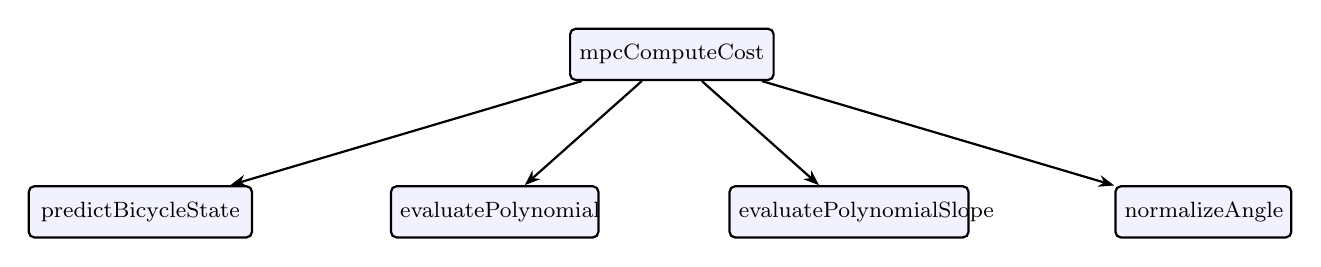
\begin{tikzpicture}[
  level 1/.style={sibling distance=4.5cm, level distance=2.0cm},
  every node/.style={rectangle, draw, rounded corners=2pt, thick,
    minimum height=0.65cm, text centered, font=\footnotesize,
    fill=blue!5},
  edge from parent/.style={draw, -{Stealth[length=2mm]}, thick}
]

\node {mpcComputeCost}
  child { node[text width=2.6cm] {predictBicycleState} }
  child { node[text width=2.4cm] {evaluatePolynomial} }
  child { node[text width=2.8cm] {evaluatePolynomialSlope} }
  child { node[text width=2cm] {normalizeAngle} };

\end{tikzpicture}
\end{center}

% ============================================================
%  1.7.x 下级函数需求
% ============================================================
\subsubsection{predictBicycleState~---~自行车模型状态预测}

\begin{itemize}
  \item \textbf{功能}：基于运动学自行车模型，使用欧拉前向离散预测下一时刻车辆状态。
  \item \textbf{输入}：\texttt{VehicleState}（当前状态）、\texttt{ControlInput}（控制输入）、\texttt{dt}（时间步长）、\texttt{wheelbase}（轴距）。
  \item \textbf{输出}：\texttt{VehicleState}（下一时刻状态）。
  \item \textbf{算法}：$x_{k+1} = x_k + v_k \cos\psi_k \cdot \Delta t$，$y_{k+1} = y_k + v_k \sin\psi_k \cdot \Delta t$，$\psi_{k+1} = \psi_k + v_k \tan\delta_k / L \cdot \Delta t$，$v_{k+1} = v_k + a_k \cdot \Delta t$。
\end{itemize}

\subsubsection{evaluatePolynomial~---~多项式求值}

\begin{itemize}
  \item \textbf{功能}：使用 Horner 法计算 $y = c_0 + c_1 x + c_2 x^2 + c_3 x^3$。
  \item \textbf{输入}：\texttt{PolynomialCoeffs}（系数）、\texttt{x}（double）。
  \item \textbf{输出}：double（多项式值）。
\end{itemize}

\subsubsection{evaluatePolynomialSlope~---~多项式斜率求值}

\begin{itemize}
  \item \textbf{功能}：计算三次多项式一阶导数 $dy/dx = c_1 + 2c_2 x + 3c_3 x^2$。
  \item \textbf{输入}：\texttt{PolynomialCoeffs}（系数）、\texttt{x}（double）。
  \item \textbf{输出}：double（斜率值）。
\end{itemize}

\subsubsection{normalizeAngle~---~角度归一化}

\begin{itemize}
  \item \textbf{功能}：将角度归一化到 $[-\pi, \pi]$ 区间，使用 $\text{atan2}(\sin\theta, \cos\theta)$。
  \item \textbf{输入}：\texttt{angle}（double）。
  \item \textbf{输出}：double（归一化后的角度）。
\end{itemize}

% ============================================================
%  1.8 数据结构定义
% ============================================================
\subsection{数据结构定义}

以下数据结构定义于 \texttt{waypointFollowTypes.hpp}，命名空间 \texttt{waypoint\_follow}。

\subsubsection{VehicleState~---~车辆运动状态}
\begin{longtable}{|L{3.5cm}|C{2cm}|L{9.5cm}|}
\hline
\textbf{成员} & \textbf{类型} & \textbf{说明} \\
\hline
\texttt{x} & double & 纵向位置 (m) \\
\hline
\texttt{y} & double & 横向位置 (m) \\
\hline
\texttt{yaw} & double & 航向角 (rad)，逆时针为正 \\
\hline
\texttt{v} & double & 纵向速度 (m/s) \\
\hline
\end{longtable}

\subsubsection{ControlInput~---~车辆控制输入量}
\begin{longtable}{|L{3.5cm}|C{2cm}|L{9.5cm}|}
\hline
\textbf{成员} & \textbf{类型} & \textbf{说明} \\
\hline
\texttt{steeringAngle} & double & 前轮转向角 (rad)，左转为正 \\
\hline
\texttt{acceleration} & double & 纵向加速度 (m/s\textsuperscript{2})，加速为正 \\
\hline
\end{longtable}

\subsubsection{PolynomialCoeffs~---~三次多项式系数}
\begin{longtable}{|L{3.5cm}|C{2cm}|L{9.5cm}|}
\hline
\textbf{成员} & \textbf{类型} & \textbf{说明} \\
\hline
\texttt{c[4]} & double[4] & $y = c_0 + c_1 x + c_2 x^2 + c_3 x^3$ \\
\hline
\end{longtable}

\subsubsection{FittedTrajectory~---~拟合参考轨迹}
\begin{longtable}{|L{3.5cm}|C{2cm}|L{9.5cm}|}
\hline
\textbf{成员} & \textbf{类型} & \textbf{说明} \\
\hline
\texttt{poly} & PolynomialCoeffs & 归一化坐标系下的多项式系数 \\
\hline
\texttt{xOffset} & double & X坐标归一化偏移量 (m) \\
\hline
\texttt{xScale} & double & X坐标归一化缩放因子 (m) \\
\hline
\texttt{refSpeed} & double & 路点推算的参考车速 (m/s) \\
\hline
\texttt{valid} & bool & 轨迹拟合是否有效 \\
\hline
\end{longtable}

\subsubsection{MpcParam~---~MPC控制参数集}
\begin{longtable}{|L{4cm}|C{1.5cm}|C{1.5cm}|L{8cm}|}
\hline
\textbf{成员} & \textbf{类型} & \textbf{默认值} & \textbf{说明} \\
\hline
\endfirsthead
\hline
\textbf{成员} & \textbf{类型} & \textbf{默认值} & \textbf{说明} \\
\hline
\endhead
\texttt{predictionHorizon} & int & 15 & 预测步数 $N_p$ \\
\hline
\texttt{controlHorizon} & int & 5 & 控制步数 $N_c$ \\
\hline
\texttt{dt} & double & 0.1 & 预测时间步长 (s) \\
\hline
\texttt{wheelbase} & double & 2.85 & 前后轴距 (m) \\
\hline
\texttt{wLateral} & double & 50.0 & 横向偏差代价权重 $w_{\text{lat}}$ \\
\hline
\texttt{wHeading} & double & 30.0 & 航向偏差代价权重 $w_{\text{head}}$ \\
\hline
\texttt{wVelocity} & double & 5.0 & 速度偏差代价权重 $w_v$ \\
\hline
\texttt{wSteering} & double & 1.0 & 转向角控制量代价权重 $w_\delta$ \\
\hline
\texttt{wAccel} & double & 0.5 & 加速度控制量代价权重 $w_a$ \\
\hline
\texttt{wSteeringRate} & double & 100.0 & 转向角变化率代价权重 $w_{\Delta\delta}$ \\
\hline
\texttt{wAccelRate} & double & 10.0 & 加速度变化率代价权重 $w_{\Delta a}$ \\
\hline
\end{longtable}

% ============================================================
%  1.9 测试用例
% ============================================================
\subsection{测试用例}

\subsubsection{正常测试用例}

{\small
\begin{longtable}{|C{0.6cm}|L{2.2cm}|L{4.8cm}|L{4.0cm}|L{3.5cm}|}
\hline
\textbf{编号} & \textbf{场景} & \textbf{输入} & \textbf{预期输出} & \textbf{验证准则} \\
\hline
\endfirsthead
\hline
\textbf{编号} & \textbf{场景} & \textbf{输入} & \textbf{预期输出} & \textbf{验证准则} \\
\hline
\endhead
N-1 &
零控制直线 &
$\delta_k{=}0$, $a_k{=}0$, 直线轨迹, $v_0{=}v_{\text{ref}}$ &
$J \approx 0$ &
跟踪误差和控制代价均为零 \\
\hline
N-2 &
恒定转向 &
$\delta_k{=}0.1$, $a_k{=}0$, 圆弧轨迹, $v_0{=}v_{\text{ref}}$ &
$J > 0$, $J_{\text{ctrl}} > 0$ &
控制幅值代价非零 \\
\hline
N-3 &
变化率代价 &
$\delta_0{=}0.1$, $\delta_{\text{prev}}{=}0$, $a_k{=}0$ &
$J_{\text{rate}} > 0$ &
$w_{\Delta\delta}(\delta_0{-}\delta_{\text{prev}})^2 > 0$ \\
\hline
N-4 &
速度偏差 &
$\delta_k{=}0$, $a_k{=}0$, $v_0{=}10$, $v_{\text{ref}}{=}20$ &
$J_v > 0$ &
速度误差代价显著 \\
\hline
N-5 &
控制时域截断 &
$N_c{=}3$, $N_p{=}10$, 控制序列3步 &
$k \geq N_c$ 后使用 $\mathbf{u}_{N_c-1}$ &
代价有限, 无数组越界 \\
\hline
\end{longtable}
}

\vspace{6pt}
{\small
\begin{longtable}{|L{2.5cm}|L{13cm}|}
\hline
\multicolumn{2}{|c|}{\textbf{正常测试用例符号说明}} \\
\hline
\textbf{符号} & \textbf{含义} \\
\hline
$\delta_k$ & 第 $k$ 步转向角 controlSequence[$k$].steeringAngle (rad) \\
\hline
$a_k$ & 第 $k$ 步加速度 controlSequence[$k$].acceleration (m/s\textsuperscript{2}) \\
\hline
$\delta_{\text{prev}}$ & 上周期转向角 prevAppliedControl.steeringAngle (rad) \\
\hline
$v_0$ & 初始车速 initialState.v (m/s) \\
\hline
$v_{\text{ref}}$ & 参考车速 trajectory.refSpeed (m/s) \\
\hline
$J$, $J_{\text{ctrl}}$, $J_{\text{rate}}$, $J_v$ & 总代价 / 控制幅值代价 / 变化率代价 / 速度代价 \\
\hline
$N_p$, $N_c$ & 预测步数 / 控制步数 \\
\hline
\end{longtable}
}

\subsubsection{异常测试用例}

{\small
\begin{longtable}{|C{0.6cm}|L{2.0cm}|L{4.5cm}|L{4.2cm}|L{3.8cm}|}
\hline
\textbf{编号} & \textbf{场景} & \textbf{输入} & \textbf{预期输出/行为} & \textbf{验证准则} \\
\hline
\endfirsthead
\hline
\textbf{编号} & \textbf{场景} & \textbf{输入} & \textbf{预期输出/行为} & \textbf{验证准则} \\
\hline
\endhead
A-1 &
NaN 初始状态 &
$v_0{=}\text{NaN}$, 其余正常 &
不崩溃; $J$ 可能为 NaN &
函数正常返回 \\
\hline
A-2 &
Infinity 速度 &
$v_0{=}+\infty$ &
预测状态发散; $J{=}+\infty$ &
函数返回, 不崩溃 \\
\hline
A-3 &
NaN 转向角 &
$\delta_0{=}\text{NaN}$ &
tan(NaN) 传播; $J$ 含 NaN &
函数正常返回 \\
\hline
A-4 &
零 xScale &
\texttt{trajectory.xScale}{$= 0$} &
归一化除零; $\bar{x}_k{=}\pm\infty$ &
不崩溃, $J$ 可能无穷 \\
\hline
A-5 &
负 xScale &
\texttt{trajectory.xScale}{$= -1$} &
归一化方向反转 &
函数返回有限代价 \\
\hline
A-6 &
Infinity 权重 &
$w_{\text{lat}}{=}+\infty$ &
任何非零横向误差导致 $J{=}\infty$ &
函数返回, 不崩溃 \\
\hline
A-7 &
零轴距 &
\texttt{wheelbase}{$= 0$} &
$\dot\psi = v\tan\delta / 0$ 除零 &
函数返回, 不崩溃 \\
\hline
A-8 &
极大转向角 &
$\delta_k{=}\pi/2$ (tan 趋无穷) &
$\tan(\pi/2)$ 极大, 状态发散 &
函数返回有限/无穷代价 \\
\hline
A-9 &
$N_p{=}0$ 预测步数 &
\texttt{predictionHorizon}{$= 0$} &
循环不执行, $J{=}0$ &
返回 $J{=}0.0$ \\
\hline
A-10 &
$N_c > N_p$ &
$N_c{=}10$, $N_p{=}5$ &
$k < N_c$ 条件在 $k \geq N_p$ 后不执行 &
代价有限, 逻辑正确 \\
\hline
\end{longtable}
}

\vspace{6pt}
{\small
\begin{longtable}{|L{2.5cm}|L{13cm}|}
\hline
\multicolumn{2}{|c|}{\textbf{异常测试用例符号说明}} \\
\hline
\textbf{符号} & \textbf{含义} \\
\hline
$v_0$ & 初始车速 initialState.v (m/s) \\
\hline
$\delta_k$ & 第 $k$ 步转向角 (rad) \\
\hline
$\bar{x}_k$ & 归一化后的纵向坐标 \\
\hline
$J$ & MPC总代价值 \\
\hline
$w_{\text{lat}}$ & 横向偏差代价权重 wLateral \\
\hline
$N_p$, $N_c$ & 预测步数 / 控制步数 \\
\hline
NaN & IEEE 754 非数值 (Not a Number) \\
\hline
$+\infty$ & IEEE 754 正无穷大 \\
\hline
\end{longtable}
}

\end{document}
